\documentclass{beamer}
\usepackage[utf8x]{inputenc}
\usepackage{hyperref}
\usepackage[footheight=1em]{beamerthemeboxes}
%\usepackage{pgfpages}
%\setbeameroption{show notes on second screen=left}
\usetheme{Singapore}

%\usetheme{Frankfurt}


%\addfootboxtemplate{\color{white}}{\color{gray}
  %\insertframenumber/\inserttotalframenumber\null}



%\setbeamertemplate{background canvas}{\includegraphics
%   [width=\paperwidth,height=\paperheight]{img/fond.png}}


\title{Analyse et implémentation d'un modèle de conscience artificielle}
\subtitle{Travail d'Étude et de Recherche \\ Master Informatique 1\ière année (GMIN20B)}
\author{William Dyce \and Thibaut Marmin \\ Namrata Patel \and Clément Sipieter}
\institute{Université Montpellier 2\\Encadré par Violaine Prince et Guillaume Tisserant}
\date{7 mai 2012}

\begin{document}

\AtBeginSection[]
{
  \begin{frame}{Analyse et implémentation d'un modèle de conscience artificielle}
  \begin{columns}[t]
  \begin{column}{5cm}
  \tableofcontents[sections={1-3},currentsection,hideothersubsections]
  \end{column}
  \begin{column}{5cm}
  \tableofcontents[sections={4-6},currentsection,hideothersubsections]
  \end{column}
  \end{columns}
  \end{frame}
}

\begin{frame}
\titlepage
\end{frame}

\begin{frame}{Analyse et implémentation d'un modèle de conscience artificielle}
    

  \begin{columns}[t]
  \begin{column}{5cm}
  \tableofcontents[sections={1-3},hideallsubsections]
  \end{column}
  \begin{column}{5cm}
  \tableofcontents[sections={4-6},hideallsubsections]
  \end{column}
  \end{columns}

\end{frame}

\section{Introduction}
%--------------------------------------------------------------------------------
% A COGNITIVE SYSTEM
%--------------------------------------------------------------------------------
\begin{frame}{Introduction}{A "cognitive" system}

"How can FCA  optimise a cognitive memory  structure?"

Cognition:
"The mental action or process of acquiring knowledge and understanding through thought, experience, and the senses."
Oxford Dictionary

\end{frame}

%--------------------------------------------------------------------------------
% LEARNING FROM EXPERIENCE
%--------------------------------------------------------------------------------
\begin{frame}{Introduction}{Pattern-matching for knowledge generalisation}

An unfamilliar object can be evaluated by looking at attributes shared with objects for which the value is known.

Objects pass their value to their attributes, attributes pass this value on to other objects.

\end{frame}

%--------------------------------------------------------------------------------
% SYTEM LIMITATIONS
%--------------------------------------------------------------------------------
\begin{frame}{Introduction}{System limitations}

The value of an object may derive from a specific combination of attributes which, independtly, would not have 
any particular value.

\end{frame}

%--------------------------------------------------------------------------------
% HOW FCA CAN HELP
%--------------------------------------------------------------------------------
\begin{frame}{Introduction}{How FCA can help}

FCA allows as to evaluate concepts as well as objects and attributes, and so to reason at a higher level of
abstraction.

\end{frame}

\section{Analyse Générale}
\subsection{Contraintes de réalisation}
\begin{frame}{Contraintes de réalisation}{Temporelle , d'effectifs et de
compétences}
\begin{itemize}
  \item Temps : travail à réaliser en trois mois
  \item Effectif : quatre membres dans l'équipe
  \item Compétences :
  \begin{itemize}
    \item Compétences requises à la \textbf {fin} du semestre \newline =
    Compétences nécessaires pour la réalisation du projet
    \end{itemize}
\end{itemize}
\end{frame}


\subsection{Restrictions appliquées au modèle}
\begin{frame}{Restrictions appliquées au modèle}{Environnement , fonctionnement}
\begin{tabular}{l l}
\begin{minipage}{0.6\textwidth}\begin{center}
\includegraphics[width=\textwidth]{img/analyse_generale/modele_restraint}
\end{center}\end{minipage} & \begin{minipage}{0.4\textwidth}
\begin{itemize}
  \item \textbf{Environnement : }Limitation à un type précis de jeu
  \item \textbf{Fonctionnement : }Retrait et simulation des parties
  \begin{itemize}
    \item Retrait de la métamnèse
    \item Simulation de la partie inconsciente
  \end{itemize}
\end{itemize}
\end{minipage}
\end{tabular}
\end{frame}


\subsection{Domaine d'application}
%----------------------------------------
% DOMAINE D'APPLICATION : POUQUOI
%----------------------------------------
\begin{frame}{Domaine d'application}{Jeu de plateau}

\begin{block}{Pourquoi le jeu de plateau ?}
\begin{itemize}
\item Convergence \texttt{DECOL} / \texttt{IMAGINA}
\pause
\item Activité purement cognitive
\pause
\item Activité cognitive complète
\pause
\item Évaluation facile de la performance
\end{itemize}
\end{block}

\end{frame}


%----------------------------------------
% LE MINIMAX
%----------------------------------------
\begin{frame}{Domaine d'application}{Théorie des jeux}

\begin{block}{Théorème du MiniMax}
\begin{itemize}
\item J. Von Neumann, 1928
\item \textit{Stratégie optimale pour un joueur donné}
\end{itemize}
\end{block}
\end{frame}


%----------------------------------------
% LIMITES DU MINIMAX
%----------------------------------------

\begin{frame}{Domaine d'application}{Limites du MiniMax}

\begin{block}{Types de confrontation}
\begin{itemize}
\item jeux compétitifs,
\item à deux joueurs,
\item à somme nulle,
\item durée, nombre d'options finis.
\end{itemize}
\end{block}

\pause

\begin{block}{Temps de calcul}
\begin{itemize}
\item En moyenne \emph{$O(b^{\frac{d}{2}})$} :
	\begin{itemize}
	\item d : longueur de la partie.
	\item b : nombre options par tour.
	\end{itemize}
\item En pratique : besoin d'heuristiques $\Rightarrow$ perte d'optimalité
\end{itemize}
\end{block}

\end{frame}

\section{Analyse \& Implémentation}
\subsection{Environnement \& simulation}
\begin{frame}{Environnement \& Simulation}{L'arbitre}
Environnement "arbitre" du jeux (séparation des agents de l'environnement)
\end{frame}

\begin{frame}{Environnement \& Simulation}{Librairie \texttt{game\_logic}}

\end{frame}

\begin{frame}{Environnement \& Simulation}{Web service \texttt{game\_service}}
\begin{itemize}
\item Java Servlet Technology
\item Representationnal State Transfer (HTTP,XML)
\end{itemize}
\end{frame}

\begin{frame}{Environnement \& Simulation}{Client Humain}
\begin{itemize}
\item JQuery
\item AJAX polling
\end{itemize}
\end{frame}

\begin{frame}{Environnement \& Simulation}{Client machine frontière}

\end{frame}




\subsection{Généralités}
\begin{frame}{Généralités}{Séquence d'un coup}
modified simplified general diagram
\end{frame}



\subsection{Analyseur conceptuel}
\begin{frame}{Analyseur conceptuel}{Généralités}
\begin{itemize}
  \item Représente les connaissances tirées de l'environnement
  \item Analyse ces connaissances afin d'en tirer des nouvelles
\end{itemize}
\end{frame}

\begin{frame}{Analyseur conceptuel}{Analyse détaillée}
\begin{itemize}
  \item Représentation des connaissances : \textbf{vocabulaire}
  \begin{itemize}
    \item Graphes conceptuels de base ou
    \item Formules de logique du premier ordre
  \end{itemize}
  \item Analyse des connaissances : \textbf{mécanisme}
  \begin{itemize}
    \item Interrogation avec la mémoire
    \item Recherche d'homomorphismes
  \end{itemize}
\end{itemize}
\end{frame}

\begin{frame}{Analyseur conceptuel}{Implémentation : Rôles du module}
\begin{itemize}
  \item Convertisseur :
  \begin{itemize}
    \item Rend les données de l'environnement \enquote{lisibles} par l'IA
  \end{itemize}
  \item Moteur d'inférence :
  \begin{itemize}
    \item Applique les règles générés par l'IA afin d'en
    sortir des nouveaux concepts
  \end{itemize}
\end{itemize}
\end{frame}

\begin{frame}{Analyseur conceptuel}{Implémentation : Classes principales}
\begin{itemize}
  \item \textbf {Choices (environnement)} : représente un plateau
  courant, un coup et l'ensemble des plateaux résultants de ce coup
  \item \textbf {BoardMatrix(environnement)} : représente un plateau en forme
  d'une matrice
  \item \textbf {Choices\_FOL (IA)} : version logique du premier ordre de
  Choices (même structure, attributs décrits par des formules logiques)
  \item \textbf {CompleteBoardState (IA)} : version logique du premier ordre de
  BoardMatrix (classe qui décrit la configuration
  d'un plateau complet comme une liste de faits logiques)
  \item \textbf {RelevantPartialBoardState (IA)} : classe qui décrit la
  configuration d'une sous-partie pertinante d'un plateau comme une règle
  logique
\end{itemize}
\end{frame}


\begin{frame}{Analyseur conceptuel}{Implémentation détaillée}
\begin{itemize}
  \item \textbf {Convertisseur} :
  \begin{itemize}
    \item Entrée (de l'environnement): instance de \enquote{Choices}
    \item Algorithme qui transforme un \enquote{BoardMatrix} en un
    \enquote{CompleteBoardState}
    \item Sortie: instance de
    \enquote{Choices\_FOL}
  \end{itemize}
  \item \textbf {Moteur d'inférence} :
  \begin{itemize}
    \item Entrée (de la mémoire) : instance de
    \enquote{RelevantPartialBoardState}
    \item Algorithme de saturation de la base de faits des
    \enquote{CompleteBoardState} par la règle d'entrée
    \item Ajout d'une liste de \enquote{RelevantPartialBoardState} présents dans
    chaque \enquote{CompleteBoardState} du pacquet \enquote{Choices\_FOL}
    \item Sortie (passée à la mémoire) : instance de
    \enquote{Choices\_FOL}
  \end{itemize}
\end{itemize}
\end{frame}


\subsection{Raisonneur}
\begin{frame}{Raisonneur}{Moteur de choix}
Proba / Bayes
\end{frame}

\begin{frame}{Raisonneur}{Moteur d'introspection}
Comparaison de représentation mémorisé de l'environnement, afin d'en extraire des sous partie commune (RPBS)
\end{frame}

\subsection{Mémoire}
\begin{frame}{Mémoire}{Interface Mémoire}
\begin{center}
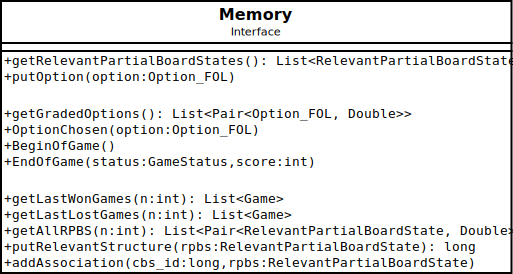
\includegraphics[width=0.7\textwidth]{img/implementation_memory/interface}
\end{center}
\end{frame}

\begin{frame}{Mémoire}{Persistance}
\begin{center}
\includegraphics[width=0.3\textwidth]{img/neo4j/neo4j_logo}
\end{center}
\begin{block}{Neo4j}
\begin{itemize}
\item Logiciel libre (GPLv3 / AGPLv3)
\item SGBD NoSQL orienté graphe
\item Respect des caractéristiques ACID
\item Multiple versions (embedded in Java)
\end{itemize}
\end{block}
\end{frame}

\begin{frame}{Mémoire}{Persistance}
\begin{block}{Élements}
\begin{itemize}
\item Noeud racine
\item Noeuds
\item Relations (orientées)
\item Types de relations
\item Attributs (Noeuds \& Relations)
\end{itemize}
\end{block}
\begin{block}{Comment typer les noeuds ?}
\begin{enumerate}
\item Créer un noeud \texttt{Maitre}
\item Créer une relation typée \texttt{Racine $\rightarrow$ Maitre}
\item Créer des relations typées \texttt{Maitre $\rightarrow$ Noeuds}
\end{enumerate}
\end{block}
\end{frame}

\subsection{Conclusion partielle}
\begin{frame}{Optimisation}{Structures de données}

\end{frame}

\begin{frame}{Optimisation}{MultiThreading}

\end{frame}

\begin{frame}{Optimisation}{Autre}

\end{frame}


\section{Outils de travail}
\subsection{Rédaction collaborative}
\begin{frame}{Outils de travail}{Etherpad - Éditeur de texte collaboratif}
\begin{center}
	\includegraphics[width=0.3\textwidth]{img/outils/etherpad}\\
\end{center}
\begin{tabular}{l l}
\begin{minipage}{0.5\textwidth}\begin{center}
\includegraphics[width=\textwidth]{img/outils/etherpad_screenshot}\\
\textit{\tiny Aperçu d'un pad hébergé sur \texttt{framapad.org}}
\end{center}\end{minipage} & \begin{minipage}{0.5\textwidth}
\begin{itemize}
\item Logiciel libre

\textit{Licence Apache v2}
\item Collaboratif en temps réel
\item Complet

\textit{Chat, couleurs, etc.}
\item Hébergement via Framapad
\texttt{\small http://framapad.org/}
\end{itemize}
\end{minipage}
\end{tabular}
\end{frame}

\subsection{Gestionnaire de versions}
\begin{frame}{Outils de travail}{GIT - Un gestionnaire de version décentralisé}
\begin{tabular}{l r}
\begin{minipage}{0.5\textwidth}
\includegraphics[width=0.7\textwidth]{img/outils/git}\\
\begin{itemize}
\item Logiciel libre (GNUv2)
\item Simple d'utilisation
\item Hébergement via GitHub
\texttt{\small https://github.com/cogitoTeam/artificial\_consciousness/}
\end{itemize}
\end{minipage} & \begin{minipage}{0.5\textwidth}\begin{center}
\includegraphics[width=0.2\textwidth]{img/outils/github_logo} \\
\includegraphics[width=0.5\textwidth]{img/outils/github_octocat}
\end{center}
\end{minipage}
\end{tabular}
\end{frame}

\subsection{Développement}
\part{Développement}
\minitoc


\chapter{Spécifications techniques}

\section{Environnement}

\input{developpement/specifications_techniques/archi}

\section{L'agent \og Cogito \fg{} }

\input{developpement/specifications_techniques/generales}

\section{Analyse}

\input{developpement/specifications_techniques/analyse}

\section{Raisonnement}

\input{developpement/specifications_techniques/raisonnement}

\section{Mémoire}

\input{developpement/specifications_techniques/memoire}

\chapter{Méthode de travail}

\section{Répartition des tâches}

Dans le but de pouvoir travailler séparément et de manière autonome sur chaque module lors de l'implémentation, nous avons rigoureusement travaillé les spécifications techniques et l'architecture globale de l'application. Les tâches de développement ont ensuite été  menées de manière parallèle par chacun des membres de l'équipe :

\begin{itemize}
\item Namrata était résponsable du module d'analyse,
\item Clément du raisonnement,
\item Thibaut de la mémoire,
\item et William de l'environnement et du serveur de jeu.
\end{itemize}   

Nous nous sommes réunis tout au long du développement pour assurer l'avancement global du projet et répondre aux interrogations de chacun.

\section{Outils utilisés}

\subsection{Gestionnaire de versions}
Tout au long du projet, nous avons utilisé \emph{git} : un gestionnaire de version décentralisé. Un tel outil permet la mise en commun des travaux, la gestion des versions et la gestion des \emph{merges}\footnote{Fusion de deux fichiers différents.}. 

\begin{center}
	\includegraphics[width=0.3\textwidth]{files/outils/git}	
\end{center}

Nous avons choisi \emph{git} pour plusieurs raisons :

\begin{itemize}
\item plutôt simple d'utilisation (par rapport à ses homologues comme \emph{SVN}),
\item hébergement gratuit via GitHub (sous condition de diffusion du code sous une licence libre),
\item \emph{git} est une solution libre sous licence \gls{GPLv2}.
\end{itemize}

\subsection{EtherPad, un éditeur de texte collaboratif}
\emph{EtherPad} se présente sous la forme d'un éditeur de texte léger permettant de faire un minimum de mise en page.

\begin{figure}[H]
	\includegraphics[width=\textwidth]{files/outils/etherpad_screenshot}	
	\caption{Aperçu de l'interface d'\emph{EtherPad} hébergé sur \emph{framapad} (site mis à disposition par Framasoft utilisant le code d'EtherPad).}
	\label{etherpad_screenshot}
\end{figure}

\begin{center}
\includegraphics[width=0.4\textwidth]{files/outils/etherpad}
\end{center}

L'interface d'\emph{EtherPad} se présente sous la forme d'une interface web (figure \ref{etherpad_screenshot}) où chaque utilisateur connecté possède une couleur. La singularité de cet outil réside dans le fait que toutes les modifications effectuées sur le pad sont visibles par tous en temps réel.

Un chat est également disponible ce qui facilite la collaboration entre les utilisateurs connectés.

Il est important de noter qu'\emph{EtherPad} est sous licence \gls{Apache v2}.

\subsection{Visualisation de graphes}

Pour débugger la base de données Neo4j, nous avons utilisé \emph{Gephi}, un utilitaire basé sur la \emph{NetBeans Platform}.

\begin{center}
\includegraphics[width=0.4\textwidth]{files/outils/gephi}
\end{center}

Il permet de visualiser et de manipuler des graphes. C'est un outil libre qui embarque quelques plugins dont un connecteur Neo4j permettant l'import de bases de données du SGBD.

\subsection{Outils de développement}
Voici une liste non exhaustive des outils que nous avons utilisés lors de nos développements :
\begin{description}
\item[Eclipse / NetBeans] Il s'agit des deux principaux EDI\footnote{Environnement de Développement Intégré} libres.
\item[Javadoc] Nous avons pris soin de documenter la totalité de notre code dans le but de rentre notre code réutilisable. Javadoc est aujourd'hui devenu un standard industriel utilisé par la majorité des développement Java.
\item[Log4j] Librairie Java libre qui permet la journalisation sous formes variées (stdout\footnote{Flux de sortie standard.}, fichiers de log, envoie de mail, etc.).
\item[YourKit Java Profiler] Afin de permettre d'optimiser certaines méthodes, nous avons utilisé cet outil en version d'évaluation (sous licence propriétaire). Il s'intègre parfaitement dans la plupart des environnement de développement.
\end{description}

\section{Conclusion \& Perspectives}
\subsection{Conclusion}
\begin{frame}{Optimisation}{Structures de données}

\end{frame}

\begin{frame}{Optimisation}{MultiThreading}

\end{frame}

\begin{frame}{Optimisation}{Autre}

\end{frame}

\subsection{Perspectives}
\begin{frame}{Perspectives}
Ce qui (n') a (pas) été réussi
Sacrifices faits (système opérationelle)
Problèmes rencontrés (NP-complétude)
Forces et faiblesses du sysème
Pistes à suivre pour une suite éventuelle
Évaluation du système à faire
\end{frame}

\section*{Demonstration \& Questions}
\begin{frame}{Merci pour votre attention}{Questions \& Démo}
\vspace*{\stretch{1}}
\texttt{https://github.com/cogitoTeam/IA\_a\_cognitive\_approach}

\end{frame}

\end{document}